\documentclass{article}
\usepackage[margin=.3in]{geometry}
\usepackage{tikz}
\usetikzlibrary{shapes, arrows.meta} 
\usepackage{amsmath}
\newcommand{\tuple}[1]{\ensuremath{\left\langle #1 \right\rangle}}

\begin{document}

\textbf{Exercice 7}

A)
\[
\left(
\begin{array}{*{12}{c}}
0 & 1 & 1 & 0 & 0 & 1 & 0 & 0 & 0 & 0 & 0 & 0\\
1 & 0 & 1 & 0 & 0 & 0 & 0 & 0 & 0 & 0 & 0 & 0\\
1 & 1 & 0 & 1 & 0 & 0 & 0 & 0 & 0 & 0 & 0 & 0\\
0 & 0 & 1 & 0 & 1 & 0 & 0 & 0 & 1 & 0 & 0 & 0\\
0 & 0 & 0 & 1 & 0 & 1 & 0 & 1 & 0 & 0 & 0 & 0\\
1 & 0 & 0 & 0 & 1 & 0 & 1 & 0 & 0 & 0 & 0 & 0\\
0 & 0 & 0 & 0 & 0 & 1 & 0 & 1 & 0 & 0 & 0 & 1\\
0 & 0 & 0 & 0 & 1 & 0 & 1 & 0 & 1 & 0 & 0 & 0\\ 
0 & 0 & 0 & 1 & 0 & 0 & 0 & 1 & 0 & 1 & 0 & 0\\ 
0 & 0 & 0 & 0 & 0 & 0 & 0 & 0 & 1 & 0 & 1 & 0\\ 
0 & 0 & 0 & 0 & 0 & 0 & 0 & 0 & 0 & 1 & 0 & 1\\
0 & 0 & 0 & 0 & 0 & 0 & 1 & 0 & 0 & 0 & 1 & 0\\
\end{array}
\right)
\]
\vspace{0.1cm}

B)
Avec les labels pour les sommets comme $v_i$ pour les faces comme $f_i$ et les arêtes comme $e_i$, où $0 \leq v_i \leq 17$, $1 \leq f_i \leq 9$, 

et $1 \leq e_i \leq 25$, on peut observer la formule d'Euler pour ce graphe planaire $G_5$

$$|V(G_5)| + |F(G_5)|- |E(G_5)| = 18 + 9 - 25= 2$$

\begin{center}
    \begin{minipage}{0.3\textwidth}
        \begin{tikzpicture}[transform canvas={shift={(1, -3)}}]
            \node[circle, draw, minimum size=0.7cm] (n0) at (-4, 0) {$v_0$};
            \node[circle, draw, minimum size=0.7cm] (n1) at (-6, 1) {$v_1$};
            \node[circle, draw, minimum size=0.7cm] (n2) at (-4, 2) {$v_2$};
            %V(G1)
            \node[circle, draw, minimum size=0.7cm] (n3) at (-2, 3) {$v_3$};
            \node[circle, draw, minimum size=0.7cm] (n4) at (-2, 1) {$v_4$};
            \node[circle, draw, minimum size=0.7cm] (n5) at (-2, -1) {$v_5$};
            %V(G2)
            \node[circle, draw, minimum size=0.7cm] (n8) at (0, 3) {$v_8$};
            \node[circle, draw, minimum size=0.7cm] (n7) at (0, 1) {$v_7$};
            \node[circle, draw, minimum size=0.7cm] (n6) at (0, -1) {$v_6$};
            %V(G3)
            \node[circle, draw, minimum size=0.7cm] (n9) at (2, 3) {$v_9$};
            \node[circle, draw, minimum size=0.7cm] (n10) at (2, 1) {$v_{10}$};
            \node[circle, draw, minimum size=0.7cm] (n11) at (2, -1) {$v_{11}$};
            %V(G4)
            \node[circle, draw, minimum size=0.7cm] (n14) at (4, 3) {$v_{14}$};
            \node[circle, draw, minimum size=0.7cm] (n13) at (4, 1) {$v_{13}$};
            \node[circle, draw, minimum size=0.7cm] (n12) at (4, -1) {$v_{12}$};
            %V(G5)
            \node[circle, draw, minimum size=0.7cm] (n17) at (6, 3) {$v_{17}$};
            \node[circle, draw, minimum size=0.7cm] (n16) at (6, 1) {$v_{16}$};
            \node[circle, draw, minimum size=0.7cm] (n15) at (6, -1) {$v_{15}$};
            %E(G0)
            \draw[-, thick] (n0) -- (n1) node[midway, below] {$e_1$};
            \draw[-, thick] (n1) -- (n2) node[midway, above] {$e_2$};
            \draw[-, thick] (n2) -- (n0) node[midway, left] {$e_3$};
            %E(G1) - E(G0)
            \draw[-, thick] (n2) -- (n3) node[midway, above] {$e_4$};
            \draw[-, thick] (n3) -- (n4) node[midway, left] {$e_5$};
            \draw[-, thick] (n4) -- (n5) node[midway, left] {$e_6$};
            \draw[-, thick] (n5) -- (n0) node[midway, below] {$e_7$};
            %E(G2) - E(G1)
            \draw[-, thick] (n3) -- (n8) node[midway, above] {$e_8$};
            \draw[-, thick] (n8) -- (n7) node[midway, right] {$e_9$};
            \draw[-, thick] (n7) -- (n6) node[midway, right] {$e_{11}$};
            \draw[-, thick] (n6) -- (n5) node[midway, below] {$e_{12}$};
            \draw[-, thick] (n4) -- (n7) node[midway, above] {$e_{10}$};
            %E(G3) - E(G2)
            \draw[-, thick] (n8) -- (n9) node[midway, above] {$e_{13}$};
            \draw[-, thick] (n9) -- (n10) node[midway, left] {$e_{14}$};
            \draw[-, thick] (n10) -- (n11) node[midway, left] {$e_{15}$};
            \draw[-, thick] (n11) -- (n6)  node[midway, below] {$e_{16}$};
            %E(G4) - E(G3)
            \draw[-, thick] (n9) -- (n14)  node[midway, above] {$e_{17}$};
            \draw[-, thick] (n14) -- (n13) node[midway, right] {$e_{18}$};
            \draw[-, thick] (n13) -- (n12) node[midway, right] {$e_{20}$};
            \draw[-, thick] (n12) -- (n11) node[midway, below] {$e_{21}$};
            \draw[-, thick] (n10) -- (n13) node[midway, above] {$e_{19}$};
            %E(G5) - E(G4)
            \draw[-, thick] (n14) -- (n17) node[midway, above] {$e_{22}$};
            \draw[-, thick] (n17) -- (n16) node[midway, right] {$e_{23}$};
            \draw[-, thick] (n16) -- (n15) node[midway, right] {$e_{24}$};
            \draw[-, thick] (n15) -- (n12) node[midway, below] {$e_{25}$};
            % face labels
            \node at (-5, 1) {$f_1$};
            \node at (-3, 1) {$f_2$};
            \node at (-1, 2) {$f_3$};
            \node at (-1, 0) {$f_4$};
            \node at (1, 1) {$f_5$};
            \node at (3, 2) {$f_6$};
            \node at (3, 0) {$f_7$};
            \node at (5, 1) {$f_8$};
            \node at (7, 1) {$f_9$};
        \end{tikzpicture}
    \end{minipage}
\end{center}

\vspace{4.5cm}

C) (i) $G_0$ est hamiltonien et pour $i>0$ impair $G_i$ et hamiltonien.
$G_1$ est hamiltonien, en effet $\tuple{v_1,v_2,v_3,v_4,v_5,v_0,v_1}.$ 

Maintenant, tout cycle hamiltonien doit nécessairement éviter $e_3$. Cela signifie qu'ils doivent tous contenir la chaîne $\tuple{v_5,v_0,v_1,v_2,v_3}$ 

ou $\tuple{v_3,v_2,v_1,v_0,v_5}$. 

Pour $n$ pair, essayons de construire un cycle pour les 3 plus grands sommets par indice. La chaîne $\tuple{v_{3n-3},v_{3n-2},v_{3n-1},...,v_3}$ 

saute $v_{3n+2}$ tandis que la chaîne $\tuple{v_{3n-3},v_{3n+2},v_{3n-1},...,v_3}$ saute $v_{3n-2}$. On peut raisonner de manière similaire pour les chaînes 

$\tuple{v_{3n+1},...,v_5}$ et ainsi, il n'y a pas de cycle hamiltonien pour $n$ pair.
Pour $n$ impair, construisons un cycle de manière récursive. 

On a la chaîne

$$C = \tuple{v_{3n + 1},v_{3n + 2},v_{3n - 3},v_{3(n-1) + 1},v_{3(n-1) - 2},v_{3(n-1) - 1},v_{3(n-2) + 1}, ... , v_4,v_5,v_0}$$

En remarquant que cela est possible car $n-1$ est pair. Maintenant, on a également la chaîne 

$$C^{\prime} = \tuple{v_{3n},v_{3(n-1) + 2},v_{3(n-1)},v_{3(n-2) + 2}, ...,v_8, v_3,v_2,v_1}$$

Par conséquent, $C \circ (C^{\prime})^{-1}$ est un cycle hamiltonien.



(ii) $G_0$ est eulérien. Cependant, pour $i>0$  le sommet $v_4$ aura un nombre impair d'arêtes et ne peut donc pas 

être eulérien.

(iii) $G_0$ est complet mais pour $i > 0$, $G_i$ sont pas complets car nous pouvons voir que le sommet $v_4$ n'a 

aucun arêtes sur aucun des sommets de $G_0$

(iv)$G_0$ est regulier mais pour $i > 0$, $G_i$ sont pas reguliers car nous pouvons voir $v_1$ et $v_2$  n'ont pas le même numéro 

d'arêtes que $v_0$

(v) Aucun des graphes n'est biparti

(vi) oui

(vii) oui

(viii) oui

(ix) oui pour tout $i$, car on peut toujours supprimer $e_3$ et il restera connexe.

(x) oui pour tout $i> 1$, car on peut toujours supprimer $e_3$ et $e_5$ et il restera connexe.

(xi) oui

D)non non oui


    


\end{document}
